\documentclass[11pt]{report}
\usepackage{amsmath,amsthm,amssymb,wasysym}
\usepackage{mathtools}
\usepackage{enumerate}
\usepackage{graphicx}
\usepackage{mathpazo}
\usepackage{lmodern}
\usepackage{parskip}
\usepackage{fancyhdr}
\usepackage{wrapfig}
\usepackage{tikz}
\usepackage{hyperref}
\usepackage{listings}
\usepackage{authblk}
\lstdefinestyle{MyPythonStyle}
{
    language=Python,
    basicstyle=\footnotesize,
    numbers=left,
    stepnumber=1,
    showstringspaces=false,
    tabsize=1,
    breaklines=true,
    breakatwhitespace=false,
}
\lstdefinestyle{MyCStyle}
{
    language=[Sharp]C,
    basicstyle=\footnotesize,
    numbers=left,
    stepnumber=1,
    showstringspaces=false,
    tabsize=1,
    breaklines=true,
    breakatwhitespace=false,
}
\usepackage[linesnumbered,algoruled,boxed,lined]{algorithm2e}
\usetikzlibrary{positioning, shapes.geometric, arrows}
\tikzstyle{startstop} = [rectangle, rounded corners, text centered, draw=black, fill=red!30]
\tikzstyle{io} = [text centered]
\tikzstyle{decision} = [rectangle, text centered, draw=black]
\tikzstyle{process} = [trapezium, text centered, draw=black]
\tikzstyle{arrow} = [thick,->,>=stealth]
\newtheorem{theorem}{Theorem}
\newtheorem{defn}{Definition}
\newcommand{\Jostle}{\texttt{Jostle}}
\newcommand{\dbspace}{\mathcal{R}}
\newcommand{\featspace}{\mathcal{X}}
\renewcommand{\t}[1]{\texttt{#1}}
\lhead{Senior Thesis}
\rhead{Jacob Imola}
\cfoot{\thepage}
\pagestyle{fancy}
\begin{document}
\title{Automatic, Fine-Grained Algorithmic Choice for Differential Privacy}
\date{\today}
\author[1]{Jacob Imola}
\author[1]{Jean Yang}
\affil[1]{School of Computer Science, Carnegie Mellon University}
\maketitle
\abstract{Differential Privacy is a strong privacy guarantee that comes with a cost: noise must be added to every calculation that deals with private data. There are many different places that noise can be added which results in many algorithmic choices. Furthermore, algorithms can outperform one another in certain situations, but finding the best-perfoming algorithm is highly dependent on the private database. We propose automatically exploring different algorithms to save this burden from falling on programmers. We describe a programming language, Jostle, that will correctly determine the best algorithm during runtime via meta-machine learning while making no assumptions about the algorithms themselves. We test Jostle on private decision trees, a case study that existing methods perform poorly on. We find that that Jostle is capable of predicting the correct algorithm most of the time while automating much of the data-selection process.}

\chapter{Introduction}\label{ch:intro}
The rapid technological increase in data collection, speed, and storage has brought about revolutionary insights and ideas and will continue to do so. However, with huge amounts of private data comes the concern of preventing data from ending up in the wrong hands. In order to prevent data leakage, we must lay a strong privacy foundation and give data programmers tools for implementing privacy both quickly and correctly.

Consider a healthcare database with records like patient weight, age, genetic information, and whether they are HIV positive. Giving access rights to just the patient and their doctors protects as much privacy as possible, and developing tools for verifying information flow policies is an interesting question in its own right that has been well-studied. However, sometimes it's okay to release some statistics about the database so that a programmer can find risk factors for people who have HIV. Publicly releasing the entire database doesn't protect privacy at all, yet it would be good for society as a whole. A middle ground between these two extremes could potentially have more utility. Statistical methods exist for releasing blurry snapshots of the database, comprehensive enough so that meaningful conclusions may be drawn yet blurry enough so that individuals can be guaranteed a certain amount of privacy. However, in order to properly utilize these methods, we have to be absolutely sure that the privacy guarantee will not fail under any attack, and many attempts fail. The most promising method for doing such a disclosure is Differential Privacy~\cite{Dwork:2006}.

Differential Privacy (DP) is considered to be the gold-standard of privacy and has been researched intensely since its conception in 2005. It is a property of algorithms quantified by a real number that can be explicitly computed. Noise is the central idea: the bigger the number, the less noisy the answer and the less private the algorithm is. The unique advantage of DP is that its privacy guarantees hold with minimal assumptions about an attacker's abilities. Previous attempts at privacy were susceptible to surprise exploits that occurred after an algorithm's output was released. An output could be combined with an existing database unbeknownst to the analyst and could leak unintended informatioon. Notably, before DP, researchers were able to reidentify users in a Netflix dataset given an auxiliary dataset from IMDB and form a generalized attack against the state-of-the-art privacy algorithms of the time~\cite{Narayanan:2006}. The strong privacy guarantee of DP, on the other hand, has a rigorous mathematical foundation that makes it impervious to the post-processing attacks that compromised the Netflix dataset, and more recently, \href{https://hackernoon.com/how-to-rob-an-airbnb-252e7e7eda44}{AirBnB} and \href{https://gizmodo.com/this-is-almost-certainly-james-comey-s-twitter-account-1793843641}{Instagram}. Differential Privacy has stood the test of time as a sturdy way to protect privacy.
\begin{wrapfigure}{r}{0.5\textwidth}
\begin{center}
\includegraphics[scale=0.25]{Frontier}
\end{center}
\caption{Example privacy-accuracy frontier. Epsilon denotes the amount of privacy being released; as more privacy is released, algorithms trend toward less error.}\label{fig:frontier}
\end{wrapfigure}
However, just building a suite of DP algorithms is not satisfactory. Differential Privacy necessarily adds noise to programs, and noise adds a new layer of complexity to programs, especially when the noise is added to the middle of execution. For example, adding noise to a variable that governs how many times a loop is performed could result in two highly different program executions and thus a very noisy answer. In many DP applications, noise can be added in a number of places, different queries could be done to accomplish the same goal, and so on. A very noisy answer could potentially be avoided if the proper algorithm is deployed. If one algorithm always dominated the others, this wouldn't be much of a problem, but as we will see, the best one often depends on the database in a complex way. What we really have is a privacy-accuracy frontier populated by the various algorithms we could deploy, and we'd like to pick a Pareto-optimal algorithm. An example frontier is shown in Figure \ref{fig:frontier}. However, picking an optimal algorithm depends on extensive empirical evaluations, as theoretical bounds are often insufficient for complex algorithms~\cite{Hay:2016}. This process puts a lot of burden on the programmer, and it makes sense to automate it. Our vision is to design a privacy tool with the following properties:
\begin{enumerate}
\item \textbf{Correctness} The tool must produce results the programmer expects and not violate differential privacy in any way.
\item \textbf{Generalizability} The tool should be able to perform algorithmic choice on arbitrary code with minimal code and reasoning by the programmer.
\item \textbf{Performance} The tool should have good performance comparable to existing methods when run on the same test inputs.
\end{enumerate}
%What problem do I solve? Why is it hard? Why does it matter?
%Explain why I did decision trees.

The generality aspect of our tool is an important issue that hasn't been addressed by the literature. Currently, programmers have to do ad-hoc evaluations of algorithms to make choices, a burden that our tool will eliminate. This tool will be especially good for programmers who are privacy beginners and have no ideas about how to pick an algorithm. Our privacy tool will be able to teach such programmers about how differential privacy interacts with algorithms by showing them evidence for the best choice.

Our tool is a programming language called \Jostle{}, so named because it will ``jostle'' with different algorithms in the privacy-accuracy frontier in search of the best execution path. As a concrete example, suppose a programmer wants train a differentially private decision tree but has no idea what the frontier looks like for different algorithms. Instead of making the programmer manually evaluate the algorithms, \Jostle{} introduces the \t{ChoiceMaker} construct. This is an object that will learn how to make the right choice via machine learning, and it can be applied to any private database after creation. We designed the \t{ChoiceMaker} to automate what a data scientist does when choosing an algorithm: first collect insights or features, then train a model that does the prediction for unknown cases. In our example, the \t{ChoiceMaker} is called \t{noisyTreeChoice}, and it looks like:
\begin{lstlisting}[style=MyPythonStyle]
noisyTreeChoice = MkChoiceMaker among {DTreeAlg1, DTreeAlg2}
                    informed by {public, size}
                    trained on trainingSet 
                    with model LinRegression and ScoreFunc

answers = noisyTreeChoice(data)
\end{lstlisting}
This code has many moving parts, but it contains everything \Jostle{} needs to make an educated choice. First, the programmer provides the algorithms that he wants. Then, he must frame the learning problem to the \t{ChoiceMaker}-the purpose of the other arguments. In this case, the \t{ChoiceMaker} learns a linear regression from the space of features to the output of the \t{scoreFunc}. The features are the \t{public} properties of the database and the \t{size} of the database. Since the space of databases is huge and unstructured, features are necessary to make the learning problem tractable. The score function is any quantity that scores how an algorithm performs; for example, it could be the percentage of the decision tree's mislabeled points:
\[
scoreFunc(model, database) = \frac{1}{size}\sum_{(x, y) \in database} \mid model(x) - y\mid
\]
Finally, a \t{trainingSet} of databases must be specified for the model to learn. These databases are public databases, so privacy need not be considered when learning.

We can view the \t{ChoiceMaker} as a meta-machine learning problem as it is one step removed from running the actual algorithms. For this reason, we will start calling the features (\t{public} and \t{size}) \emph{metafeatures}. We believe that the meta-machine learning approach is a much more general way of expressing algorithmic choice than existing tools; and in fact, some existing tools reduce to this setup in the sense that they can be written as \Jostle{} programs. This is the main insight of \Jostle{}.

\paragraph{Challenges}
Performing algorithmic choice in a general setting is a difficult task as it necessitates empirical evaluation. The process of doing an empirical study is complex and difficult to automate; indeed, data scientist jobs exist and won't be automated any time soon. Any approach to this problem must balance the challenge of relieving the burden of empirical study with performance of results. It would be require no data science skills at all to just tell \Jostle{} to learn a function from the space of all databases to the best algorithm to deploy, but this problem is intractable and would likely do as poorly as deploying a random algorithm. Similarly, it is arduous yet highly performant to do an extensive study on the shape of the frontier and then deploy an algorithm with confidence. \Jostle{} takes a middle ground approach to these extremes, automating as much of deployment process as possible. Specifically, \Jostle{} automates the process of combining data science insights into a final choice and then actually running the algorithm, which is all one can hope to do under the assumption that data science cannot be automated. \Jostle{} provides the assurance that an algorithm will be chosen correctly and will perform as well as the data insights present in the metafeatures allow. 

\paragraph{Contributions} \Jostle{} is the first differentially private programming language that addresses algorithmic choice in its full generality. Therefore, it enjoys the same correctness guarantees that existing DP programming languages enjoy such as never going over budget (more on budget in Chapter \ref{ch:background}). In addition, \Jostle{} is the most general tool for algorithmic choice that we know of. Existing tools make assumptions that limit the scope in which they can be applied. Specifically, current tools cannot be applied to training private decision trees, and we perform the first automatic algorithmic choice on private decision trees with \Jostle{} to illustrate its generality. We find that \Jostle{} is capable of making the best choice for some cases of this example.

We begin with a background section on DP and related work about DP programming languages and existing tools for DP algorithmic choice. Then, we will present a formal description of how \Jostle{} works and provide an example where \Jostle{} chooses a private decision tree. Thirdly, we will implement private decision tree choice with \Jostle{} and provide empirical evidence for \Jostle{}'s decision-making ability. Finally, we make concluding remarks and discuss future directions for \Jostle{}.

\chapter{Background}\label{ch:background}
In this section, we first give a primer on differential privacy, describing the idea of budget and some simple algorithms that will be used in our example. Then, we discuss existing programming languages for differential privacy. While they don't discuss algorithmic choice, one of the languages, PINQ, will be a building block of \Jostle{}. Then, we discuss existing tools for making algorithmic choice and explain the additional constraints they impose on the algorithms.

\section{Differential Privacy Primer}
Differential Privacy makes the following promise to data subjects: ``You will not be affected, adversely or otherwise, by allowing your data to be used in any study or analysis, no matter what other studies, data sets, or information sources, are available''~\cite{Dwork:2006}. To make this more formal, we must analyze two databases, $D$ and $D'$, differing in only one row which represents a database before and after a user participates. We call such databases neighbors. Suppose we are running a algorithm $\mathcal{M}$ on the database. If an attacker is able to discern with confidence $\mathcal{M}(D)$ and $\mathcal{M}(D')$, then this poses a privacy threat. The strength of this confidence is quantified a real number $\epsilon$ such that small $\epsilon$ corresponds to low attacker confidence. This means that deterministic algorithms are already unacceptable if it's possible for $\mathcal{M}(D) \neq \mathcal{M}(D')$. We necessarily must output a probability distribution, and once we view $\mathcal{M})(D)$ as a distribution, we can finally pin down the definition:

\begin{defn}
$\mathcal{A}$ satisfies $\epsilon$-DP if for all $D$ and $D'$ such that $|D-D'|_1=1$ and for all $o$ in the range of $\mathcal{M}$, 
\[\Pr\left(\mathcal{M}(D) = o \right) \leq e^{\epsilon} \Pr\left(\mathcal{M}(D')=o\right)\]
\end{defn}

There is also a more general definition that gives a weaker privacy guarantee: 

\begin{defn}
$\mathcal{M}$ satisfies $(\epsilon, \delta)$-DP if for all $D$ and $D'$ such that $|D-D'|_1=1$ and for all $o$ in the range of $\mathcal{M}$, 
\[\Pr\left(\mathcal{A}(D) = o \right) \leq e^{\epsilon} \Pr\left(\mathcal{M}(D')=o \right) + \delta\]
\end{defn}

For much of this paper, we will focus on $\epsilon$-DP, but it is worth knowing the more general case so we can import the well-known privacy theorems in their full generality.

The definition doesn't address why the ``no matter what'' part of the promise is true, but we can view any post-release attack on $\mathcal{A}$ as a function $F$ that doesn't involve $D$. Then, the following theorem establishes the promise:

\begin{theorem}
(Post-Processing~\cite{Dwork:2006}) If $\mathcal{M}$ satisfies $(\epsilon, \delta)$-DP, and $F$ is any function that takes the output of $\mathcal{M}$ as input, then $F(\mathcal{M})$ satisfies $(\epsilon, \delta)$-DP.
\end{theorem}
This theorem is the reason why DP is such a useful guarantee. Data programmers can be sure that once they run their algorithm $\mathcal{M}$ and release its output, then the DP guarantee gets no weaker \emph{no matter what an adversary does with the data}. This prevents the headaches where a programmer realizes retroactively that the data he released can be combined in some way to reveal much more information than was intended, like in Netflix~\cite{Narayanan:2006}.

In addition, DP satisfies several other useful properties:

\begin{theorem} \label{thm:comp}
(Composition~\cite{Dwork:2006}) Given algorithm $M_1$ and $M_2$ satisfying $\epsilon_1$ and $\epsilon_2$ DP, respectively, along with a database $D$, the algorithm $M = (M_1(D), M_2(D))$ has $(\epsilon_1+\epsilon_2, \delta_1+\delta_2)$ DP.
\end{theorem}
Composition is like the union bound from probability; it's convenient to apply but often is a pessimistic bound, as we will see later. Because of composition, we often refer to $\epsilon$ as a privacy budget---if we string together many private computations, it's like we spend some of our budget on each one out of a total budget of $\epsilon$.

We can easily improve upon Composition in the special case of algorithms operating on disjoint parts of the database. If $D$ is split into disjoint parts before algorithms are applied to it, then out of all its possible neighbors, only one of the parts will be different. Thus, only the worst algorithm will affect the DP guarantee:
\begin{theorem}\label{thm:disj}
(Disjointness~\cite{Dwork:2006}) Given disjoint subsets $D_1, D_2$ of $D$ with two algorithms $M_1$ and $M_2$ providing $(\epsilon_1, \delta_1)$ and $(\epsilon_2, \delta_2)$-privacy, then $((M_1(D_1), M_2(D_2))$ satisfies $(\max\{\epsilon_1, \epsilon_2\}, \max\{\delta_1, \delta_2\})$-DP.
\end{theorem}

The most simple and commonly-used example of a DP algorithm is the Laplace mechanism. Suppose each row of our database $D$ is 0 or 1, so $D \in \{0, 1\}^n$, and that we are trying to release the sum of the elements of $D$. If this sum is $S$, then all neighboring databases $D'$ have sum $S$ or $S+1$. We can add noise to $S$ so that it looks very similar in distribution to $S+1$. The distribution we are looking for is the Laplace distribution:
\begin{defn}
The $\text{Laplace}(\lambda)$ distribution has probability mass function $f(x) = \frac{1}{2\lambda}e^{-|x|/\lambda}$.
\end{defn}
This distribution fits perfectly with the definition of DP because of the exponentials. If $X,Y$ are i.i.d. from $\text{Laplace}\left(\frac{1}{\epsilon}\right)$, then it is straightforward to show that the distributions of $S+X$ and $S+1+X$ differ by a factor of at most $e^\epsilon$ and is thus $(\epsilon, 0)$-DP. To generalize this statement, we will use the following definition:
\begin{defn}
(Sensitivity) A function $f$ is $\Delta$-sensitive if for all $x,y$ such that $|x-y|_1 = 1$, we have 
\[
|f(x) - f(y)| \leq \Delta
\]
This can equivalently be rephrased as 
\[
\max_{|x-y|_1=1}|f(x) - f(y)| = \Delta
\]
We will denote the sensitivity of $f$ by $\Delta(f)$.
\end{defn}
This gives us the following algorithm:

\begin{algorithm}\label{alg:1}
\SetAlgoLined
\SetKwInOut{Input}{Input}\SetKwInOut{Output}{Output}
\Input{$D$, a database; $f$, a function $\mathcal{D} \rightarrow \mathbb{R}^n$; and $\epsilon$}
\Output{An estimate for $f(D)$ satisfying $\epsilon$-DP.}
$X$, a vector of $n$ i.i.d. variables drawn from $\text{Laplace}\left(\frac{\Delta(f)}{\epsilon}\right)$\;
\Return{X+f(D)}
\caption{Laplace Mechanism}
\end{algorithm}

\begin{theorem}
The Laplace mechanism~\ref{alg:1} satisfies $(\epsilon, 0)$-DP~\cite{Dwork:2006}.
\end{theorem}
For the counting or histogram queries such as our example above, we have $\Delta = 1$ so we add $\text{Laplace}\left(\frac{1}{\epsilon}\right)$ noise to our function.

Another common operation is computing the maximum value in a set. If we have $n$ elements, we certainly wouldn't want to apply the Laplace mechanism $n$ times, obtaining $n\epsilon$-DP, just to have $\t{Laplace}\left(\frac{1}{\epsilon}\right)$ noise added to our answer. A better way is to use the exponential mechanism~\ref{alg:exp}.
\begin{algorithm}\label{alg:exp}
\SetAlgoLined
\SetKwInOut{Input}{Input}\SetKwInOut{Output}{Output}
\Input{$D\in \mathcal{D}$; $\mathcal{X}$, a domain; $f : \mathcal{X}\times \mathcal{D} \rightarrow \mathbb{R}$, a utility function, $\epsilon$}
\Output{$x \in \mathcal{X}$ where $f(x, D)$ is more likely to be high.}
Pick $x \in \mathcal{X}$ where $\Pr(x=k) \propto \exp\left(\frac{\epsilon f(k, D)}{2\Delta(f)}\right)$\;
\Return{$x$}
\caption{Exponential Mechanism}
\end{algorithm}
The exponential mechanism is a general algorithm that is biased towards releasing elements with higher utilities most of the time. A brief analysis shows we can pay $2\epsilon$ budget to get $\t{Laplace}\left(\frac{1}{\epsilon}\right)$-noise added to our answer as opposed to $n\epsilon$~\cite{Dwork:2006}.
\section{Related Work}
We will discuss what existing DP programming languages can do and then existing tools for making choices.
\subsection{Existing Programming Languages}
Existing programming languages for differential privacy leave algorithmic choice in the hands of the programmer. Languages with DP runtimes give the programmer certain DP primitives to use and compose them together~\cite{McSherry:2010}~\cite{Proserpio:2014}~\cite{Johnson:2017}. For example, in PINQ~\cite{McSherry:2010}, the primitives are aggregations, database splitting, and the exponential mechanism. PINQ does differential privacy bookkeeping by applying composition and disjointness to sequential applications of primitives. Privacy is kept track of with the PINQAgent. For example, the \t{NoisyCount} function is implemented in Figure~\ref{fig:PINQNoisyCount}. As we can see, PINQ will throw an error if too much privacy is used.

\begin{figure}
\begin{lstlisting}[style=myCStyle]
double NoisyCount(double epsilon){
    if(myagent.apply(epsilon)){
        return mysource.Count() + Laplace(1.0/epsilon);
    }else{
        throw new Exception("Access Denied")
    }
}
\end{lstlisting}
\caption{NoisyCount Implemented in PINQ.}
\label{fig:PINQNoisyCount}
\end{figure}

In Fuzz~\cite{Reed:2010}, a type system is implemented to guarantee differential privacy and sensitivity. Each type is endowed with a metric, and judgments are given for richer programming constructs such as sums, products, recursive types, and lambda expressions. Once the type of the program is known, its metric is known and its sensitivity can be inferred from the input variables. Sensitivity allows us to add the proper amount of noise via the Laplace mechanism. To go from an $\epsilon$-sensitive function to an $\epsilon$-DP function, noise is added via a monad by applying the function $add\_noise : \mathbb{R} \multimap M\;\mathbb{R}$.

For instance, counting the number of people in a database older than 40 could be achieved by:
\[
\lambda db.add\_noise\;(size\;(filter\;over_{40}\;db)) : db \multimap M\;\mathbb{R}
\]

The final type determined by Fuzz contains the differential privacy guarantee of the program. As opposed to throwing errors, Fuzz's sacrifice is the potential for making suboptimal typing judgments when computing the sensitivity. For instance, the sensitivity of the logarithm is infinite because its slope is unbounded, but in most cases, the slope is rather small and a better sensitivity could be added. Furthermore, its type system is undecidable.

In both of the programming languages, the programmer is still responsible for algorithmic choice. The programmer still has to decide where add noise to his computations. \Jostle{} avoids this burden by adding the algorithmic choice construct \t{ChoiceMaker}.

\subsection{Existing Methods for Algorithmic Choice}\label{sec:algchoice}

Versions of algorithmic choice have been demonstrated in previous work, but all of them make preliminary assumptions. Two of the previous works~\cite{Chaudhuri:2013}~\cite{Ligett:2017} view the problem as picking an algorithm from a set that maximizes a score function: given some answer space $\mathcal{M}$, an answer set $M \subseteq \mathcal{M}$, a database $D$, and a score function $q: \mathcal{R} \times \mathcal{M} \rightarrow \mathbb{R}$, maximize $q$ over $\mathcal{M}$ privately.

Returning to our example of private decision tree classification, $\mathcal{M}$ is the space of all decision trees and $q$ is, most commonly, a validation score on some unseen part of the database. This problem is extra subtle as changing $D$ to $D'$ changes the answer set from $M$ to $M'$, as the answers are determined on the database, and also changes $D$ to $D'$ when evaluating $q(D, m)$.

Chaudhuri and Vinterbo~\cite{Chaudhuri:2013}~\cite{Chaudhuri:2014} propose a solution based on the exponential mechanism, and directly use $q$ as the utility function used in the exponential mechanism. Since the exponential mechanism requires a sensitivity bound, a bound on $q$ must be ascertained. In order to bound $|q(D, m) - q(D', m')|$ where $m \in M$ and $m' \in M'$, two inequalities are needed:
\begin{align}
\forall m\in M,\forall |D-D'|=1:\;\|q(D, m) - q(D', m)\| &\leq \beta_1 \label{eq:sens1} \\
\forall D\in \mathcal{R},\forall m \in M,\forall m'\in M':\;\|q(D, m) -  q(D, m')\| &\leq \beta_2 \label{eq:sens2}
\end{align}

If these bounds are established, then it's relatively easy prove a bound on the output of the exponential mechanism:
\begin{theorem}\label{thm:dependent_exp}
(Utility guarantee~\cite{Chaudhuri:2013}) Let $M = m_1, m_2, \ldots, m_k$. Then, with probability at least $1-\delta$, $q(D, m_{i^*}) \geq \max_{1\leq i \leq k} q(D, m_i) - \frac{2\max\{\beta_1, \beta_2\}\log(k/\delta)}{\epsilon}$.
\end{theorem}

Going back to the decision tree example, Equation \ref{eq:sens1} forces the programmer to describe how much the validation score will change when the validation set is changed in one entry. Usually, this is not too hard; for the score function
\[
scoreFunc(model, database) = \frac{1}{size}\sum_{(x, y) \in database} \mid model(x) - y\mid
\]
this is at most $\frac{1}{size}$. However, Equation~\ref{eq:sens2} asks the programmer to bound how much the score can change when a decision tree is trained on two neighboring training databases. Because of the disrete nature of decision trees, the best a programmer can do is a bound of 1, which is quite high considering that the score function is a value betwen 0 and 1. This will produce poor performance, as the high sensitivity will overwhelm the signal contained in the score function when we apply the exponential mechanism. More details on this are given in Chapter~\ref{ch:solution}.

A different approach that still makes assumptions about algorithm sensitivity is described by Ligett et al~\cite{Ligett:2017}. The programmer decides when accuracy is sufficiently high, and privacy usage is then minimized. Critical to the framework is the method of picking correlated Laplacian noise described in~\cite{Koufogiannis:2015}. In this version of the Laplace mechanism, a programmer selects a set of increasing $\epsilon$ values, $(\epsilon_1, \epsilon_2, \ldots, \epsilon_T)$, corresponding to the different budgets they want to try. Correlated Laplace variables $(v_1, v_2, \ldots, v_T)$ are then generated such that knowing a prefix $(v_1, v_2, \ldots, v_t)$ is $\epsilon_t$-differentially private and the noise present in $v_t$ is similar to the noise that a standard Laplace mechanism would add. The framework in~\cite{Ligett:2017} uses this algorithm to add noise to models $m_1, m_2, \ldots, m_T$. Of course, the release of the most-accurate algorithm has to be done in a differentially-private manner as well, and they develop a specialized algorithm called PrivateAboveThreshold to do this. Like the first tool, this tool forces us to prove a sensitivity bound similar to Equation~\ref{eq:sens1}, and furthermore, the algorithms must be purely expressible in terms of the Laplace Mechanism, which certainly can't always be done. Decision trees are again an example of an algorithm that can't be solved with just the laplace mechanism which we will see in Chapter~\ref{ch:experiments}.

Another tool that works well for a certain case is DPComp~\cite{Hay:2016} and its extension, Pythia~\cite{Kotsogiannis:2017}. DPComp allows programmers to visualize the privacy-accuracy frontier for 2D histogram algorithms. It plots the frontier for public datasets so the programmer can deploy the proper algorithm himself. The frontier shown in Figure~\ref{fig:frontier} is actually from DPComp. The hope is that the programmer will know enough about their own dataset to manually find a similar public dataset and obtain an accurate visualization.

Pythia automates this process somewhat. Instead of making the programmer choose the proper algorithm, a decision tree based on features like database size and the number of columns in the database is created. An example decision tree appears in Figure~\ref{fig:pythia}. Pythia is quite similar to \Jostle{}---it does meta-machine learning using decision trees to predict the best 2D histogram model to deploy---but it's not a programming language. The programmer essentially must implement an ad-hoc \t{ChoiceMaker} every time he wants to do algorithmic choice. \Jostle{}'s advantage is that the \t{ChoiceMaker} is easier to implement and guaranteed to be correct.

\begin{figure}
\begin{center}
\includegraphics[scale=0.5]{PythiaDTree}
\end{center}
\caption{Example decision tree trained by Pythia with database features in branches and best algorithms in leaves.}\label{fig:pythia}
\end{figure}

\chapter{Solution Overview}\label{ch:solution}
\Jostle{} is a programming language that enforces differential privacy during the runtime like PINQ. It supports a set of DP primitives and then compositionally applies them, throwing an error whenever the privacy is used up. All interesting \Jostle{} programs will take in private databases, manipulate them in some way, and produce an answer. After the answer is calculated, differential privacy is not dealt with again due to post-processing. For instance, here is an example of a \Jostle{} program that computes the number of people in a database older than 40:
\begin{lstlisting}[style=MyPythonStyle]
def get_over_40(DB, eps):
    DB_slice = DB[row.age > 40]
    return NoisyCount(DB_slice, eps) 
\end{lstlisting}
The \t{DB[]} bracket syntax denotes database slicing, computations that can be computed with disjointness. \t{NoisyCount} denotes an aggregation that applies the Laplace mechanism (with sensitivity 1) to the size of the database, making it differentially private. While more functionality is possible, for our purposes, we will only need these two primitives as well as the exponential mechanism. So far, we have just described PINQ.

Now, we will introduce the \t{ChoiceMaker} construct. For thism we will need a more complicated example.

\section{Motivating Example}
Suppose a programmer is writing code that involves training a decision tree. They may be unsure of which of three decision tree implementations to choose for a decision tree classification problem; their choice is represented in Figure~\ref{fig:dtree_choices}. The purpose of the \t{ChoiceMaker} is to automatically make the choices for him. What we'd really love to write is something like:
\begin{lstlisting}[style=MyPythonStyle]
noisyTreeChoice = MkChoiceMaker(Alg1, Alg2, Alg3)
predictions = noisyTreeChoice(DB, epsilon)
\end{lstlisting} 
How could \Jostle{} be expected to make this choice with no other information? It has no experience on which to do a learning problem; the problem is ill-posed. We need to provide the \t{ChoiceMaker} with a training set along with a way of judging how ``good'' an algorithm is:
\begin{lstlisting}[style=MyPythonStyle]
noisyTreeChoice = MkChoiceMaker(Alg1, Alg2, Alg3)
                    trained on TrainSet with ScoreFunc
\end{lstlisting} 
This is better, as we can now define the problem as: Learn how to make the best choice given past executions of the algorithms on datasets. However, anyone in machine learning will tell us that we need to provide a hypothesis set of ``reasonable'' answers so \Jostle{} doesn't just overfit to all the examples. Thus, our code needs to be:

\begin{lstlisting}[style=MyPythonStyle]
noisyTreeChoice = MkChoiceMaker(Alg1, Alg2, Alg3)
                    trained on TrainSet 
                    with model DecisionTree and ScoreFunc
\end{lstlisting} 
Here, the hypothesis set we chose was a \t{DecisionTree}, not to be confused with the private decision trees we seek to train, but a decision tree who will predict which algorithm to deploy like Pythia's tree in Figure~\ref{fig:pythia}. However, this decision tree is learning how to go from any database at all to a predicted algorithm. The space of databases is huge and unstructured; we would need \emph{tons} of data to get any sort of good result. To fix this, we also request \emph{metafeatures} from the general ideas of what causes an algorithm to perform well or not. The database will be transformed to its metafeatures, and the model will be trained on the metafeatures instead. Our final example becomes
\begin{lstlisting}[style=MyPythonStyle]
noisyTreeChoice = MkChoiceMaker(Alg1, Alg2, Alg3)
                    informed by {size(DB), size(DB.columns)}
                    trained on TrainSet 
                    with model DecisionTree and ScoreFunc
\end{lstlisting} 
We say that the \t{ChoiceMaker} is informed by the metafeatures given by the database size and the number of columns because these metafeatures are essentially insights about algorithm performance: maybe one algorithm will work better when there isn't much data compared to the number of columns. 

We like this design because it does not sacrifice any potential for performance. If a data scientist were to work on a specific algorithmic choice instance, he would come up with good data insights which can be specified by metafeatures. A \Jostle{} program could perfectly capture the insights he gleams and could be written to execute the choice perfectly. A beginner data scientist may have no insights at all, but could just throw some simple metafeatures to a \t{ChoiceMaker} and see how they perform. For both types of programmers, \Jostle{} automates the deployment process. For a beginner, a limited amount of the data science insights process is automated as well. We now discuss the formal specification of the \t{ChoiceMaker}.

\begin{figure}
\begin{minipage}{0.5\textwidth}
\begin{center}
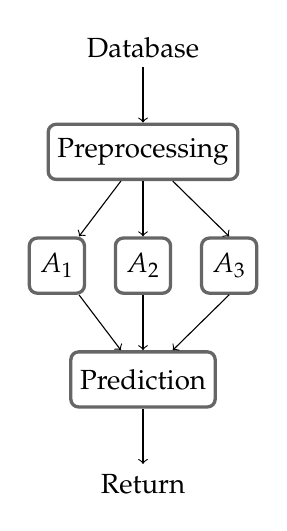
\begin{tikzpicture}[
squarednode/.style={rectangle, draw=black!60, very thick, minimum size=7mm, rounded corners=1mm},
roundnode/.style={circle, draw=black!60, very thick, minimum size=7mm}
]
\node[squarednode] (A) {Preprocessing};
\node (In) [above=2em of A] {Database};
\node[squarednode] (B2) [below=2em of A]{$A_2$};
\node[squarednode] (B1) [left=1em of B2]{$A_1$};
\node[squarednode] (B3) [right=1em of B2]{$A_3$};
\node[squarednode] (C)  [below=2em of B2]{Prediction};
\node (Out) [below=2em of C] {Return};
\draw[->] (A) -- (B1);
\draw[->] (A.south) -- (B2.north);
\draw[->] (A) -- (B3.north);

\draw[->] (B1) -- (C);
\draw[->] (B2.south) -- (C.north);
\draw[->] (B3.south) -- (C);

\draw[->] (In) -- (A);
\draw[->] (C) -- (Out);
\end{tikzpicture}
\end{center}
\end{minipage}
\begin{minipage}{0.5\textwidth}
\begin{lstlisting}[style=MyPythonStyle]
def get_preds(D, eps, test_set):
    D = Preprocess(D, eps*0.3)
    noisyTreeChoice = 
        MkChoiceMaker(Alg1, Alg2, Alg3)
            informed by {size(DB), size(DB.columns)}
            trained on TrainSet 
            with model DecisionTree and ScoreFunc

    model = noisyTreeChoice(D, eps*0.7)
    return model.predict(test_set)
\end{lstlisting}
\end{minipage}
\caption{A motivating example for \Jostle{}. A programmer may be unsure about an execution path (left side), and instead writes a \t{ChoiceMaker} to decide (right side). The privacy usage of this problem is just $\epsilon$.}\label{fig:dtree_choices}
\end{figure}
\section{Formal Description}
Let the database space be $\mathcal{R}$, the metafeature space be $\mathcal{X}$, and the answer space be $\mathcal{M}$. $\mathcal{X}$ includes a private database as well as public information such as the number of columns in the database. Any argument passed to the algorithms is also included in $\mathcal{R}$, for example, 2D histogram queries to answer. \Jostle{} uses aggregations and database splits much like PINQ. More capabilities are possible as well as long as any time private data is touched, $\epsilon$ is specified. Additionally, \Jostle{} introduces the \t{Metafeatures}, \t{Option}, and \t{Score} types, and implements constructors with the following types:

\begin{center}
\begin{tabular}{|l|p{7cm}|}
\hline
Name & Type \\ \hline
\t{Metafeatures} & $\mathcal{R} \rightarrow \mathcal{X}$ \\ \hline
\t{MkMetafeatures} & $(\mathcal{R} \rightarrow x_i) \t{ list} \rightarrow \t{Metafeatures}$ \\ \hline
\t{Option} & $\mathcal{R} \rightarrow \mathcal{M}$ \\ \hline
\t{MkOption} & $\mathcal{R} \rightarrow \mathcal{M} \rightarrow \t{Option}$ \\ \hline
\t{Score} & $\mathcal{M}\times\mathcal{R} \rightarrow \mathbb{R}$ \\ \hline
\t{MkScore} & $\mathcal{M}\times\mathcal{R} \rightarrow \mathbb{R} \rightarrow \t{Score}$ \\ \hline
\t{Model} & $\mathcal{X} \rightarrow \t{Option}$ \\ \hline
\t{MkModel} & $(\mathcal{X} \times \t{Option}) \t{ list} \rightarrow \t{Model} $\\ \hline
\t{ChoiceMaker} & $\mathcal{R} \rightarrow \mathcal{M}$ \\ \hline
\t{MkChoiceMaker} & $\t{Option list} \times \t{Metafeatures}\times \mathcal{R} \t{ list} \times \t{TrainModel} \times \t{Score} \rightarrow \t{ChoiceMaker}$ \\ \hline
\end{tabular}
\end{center}
The functions of each type and the constructors are listed below:
\begin{itemize}
\item{\t{Metafeatures}} Created by \t{MkMetafeatures} which takes in a list of functions $f_1,f_2,\ldots,f_n$ where $f_i$ has type $\mathcal{R} \rightarrow x_i$. These are the metafeature-generating functions. The metafeature space is then $\mathcal{X} = \prod_{i=1}^n x_i$. \t{MkMetafeatures} will return a function that applies all $f_i$'s to a database and return the product.
\item{\t{Option}} Created by \t{MkOption} which takes in the implementation of the algorithm that the \t{Option} represents.
\item{\t{Score}} Created by \t{MkScore} which takes in the score function. The score function tells us, given an answer and possibly using the database, how well the answer did. Usually, the score will be model performance on a validation set.
\item{\t{Model}} Created by \t{MkModel}. \t{MkModel} takes in (metafeature, algorithm pairs) and will return a \t{Model} that it learns
\item{\t{MkChoiceMaker}} Creates a \t{ChoiceMaker}. This constructor is the most complicated, and its implementation is shown in Figure \ref{fig:choicemaker}. First, models for all the inputted \t{Options} are trained. Then, a function returning the highest \t{Option} for an inputted database is returned. This function is the \t{ChoiceMaker}.
\end{itemize}

\begin{figure}
\begin{lstlisting}[style=MyPythonStyle]
def MkChoiceMaker(options, feats, train_dbs, mkmodel, score):
    xypairs = []
    for db in train_dbs:
        xypairs.append((feats(db), 
                        argmax([score(db, op(db)) for op in options])
                      ))
    model = mkmodel(xypairs)
    def GetAlg(db):
        feat = feats(db)
        return model(feats)
    return GetAlg
\end{lstlisting}
\caption{The implementation of \t{MkChoiceMaker}. }\label{fig:choicemaker}
\end{figure}

\section{Challenges}
Due to the inherent difficulty of performing automatic algorithmic choice as well as its meta-learning design, \Jostle{} presents a unique set of challenges and difficulties over other methods. First, no theoretical guarantees are able to be made about the performance of the \t{ChoiceMaker} without further assumptions unlike existing frameworks. This isn't a large problem as algorithmic choice is often solved empirically due to the highly-complex relationships of data-dependent algorithms~\cite{Hay:2016}. More seriously, \Jostle{}'s optimization is limited by the programmer's metafeatures and train databases. If poor metafeatures are inputted or if the public database set is not expansive enough, then the model will almost certainly be impoverished, and the programmer must work to improve it. Luckily, a poor model can be detected after training but before any budget is actually used. We conclude that \Jostle{} removes some of the burden of algorithmic choice from the programmer, but the burden of making a successful model still remains. This is part of the larger problem that doing learning on databases is rather intractable because of the exponential size of the database space; the generality of the \t{ChoiceMaker} forces a difficult learning task.

\section{Generality Advantage}
\Jostle{} exhibits generality that has never been explored by previous approaches. In comparison to existing algorithm frameworks, \Jostle{} makes no assumptions about the score function or the algorithms. Second, \Jostle{} is a programming language that can be represented  We go into more detail about the two types of generality below.

\subsection{Assumption-less choices}
Three existing methods for algorithmic choice~\cite{Chaudhuri:2013}~\cite{Ligett:2017}~\cite{Kotsogiannis:2017} were discussed on page \pageref{sec:algchoice}. Two of these mechanisms require the sensitivity of the score function to be known, but it may not even be possible to get a good bound. For example, a good score function to use on decision trees is the fraction of correctly classified points in the decision tree. Changing one point in the training set of a decision tree may alter the prediction of a leaf, and this could change any number of the predictions for points in the validation set. Thus, the worse-case sensitivity of this function is 100\%even though one point usually won't change the tree structure at all. Thus, the theoretical guarantees in these methods won't be powerful. The latter two frameworks additionally only work for the Laplace Mechanism, which clearly doesn't solve the general problem.

\subsection{Generality as a Programming Language}
Pythia~\cite{Kotsogiannis:2017} is a framework for producing decision trees that doesn't make any assumptions about the algorithms; in fact, its method of algorithmic choice is quite similar to the \t{ChoiceMaker}. However, Pythia does not enjoy the benefits of a programming language. While Pythia was demonstrated to be effective on a single test case, the code written was ad-hoc and had to be human-verified. One is better off using \Jostle{} every time algorithmic choice is being made because it's more automated. \Jostle{} is capable of expressing the entire Pythia framework as a program; indeed, Pythia's case study could be written as code very similar to Figure~\ref{fig:choicemaker}.

\chapter{Experiments and Implementation}\label{ch:experiments}
We will demonstrate the functionality and performance of the \Jostle{} decision tree code in Figure~\ref{fig:choicemaker}. The private decision tree literature provides a good opportunity for making algorithmic choice, and there has yet to be a framework developed for them, and as explained in Chapter~\ref{ch:solution}, less-general algorithms would likely perform worse on them. We begin with a preliminary section on Decision Trees and then discuss our experimental setup and explain why the results show that \Jostle{} works.

\section{Introduction to Private Decision Trees}\label{sec:pdtrees}
In this section, we define decision trees, and then we discuss different choices that can make when designing public decision tree algorithms. For each choice, we discuss the additional challenges that arise when making these algorithms private.

\subsection{Decision Tree Preliminaries}
Decision Trees are a powerful tool for data mining due to their high human interpretability, non-parametric design, low computational cost, ability to discover non-linear relationships among attributes, resilience to missing values, ability to handle both discrete and continuous data, and ability to handle non-binary labels~\cite{Fletcher:2016}. Throughout this section, we assume we have a database $D$ with $k$ columns. Suppose the $i$th column can take values in $\mathcal{A}_i$. We call $\mathcal{A}_i$ the attributes of column $i$. Let $c$ be the output column, or ``class'', which we are trying to predict which takes values in $\mathcal{C}$. We assume for simplicity that the $\mathcal{A}_i$ and $\mathcal{C}$ are discrete sets. A decision tree classifies points by branching on attribute $i$, forming $|\mathcal{A}_i|$ subtrees. Once certain criteria are met, no more branching occurs, and instead a leaf node predicts the class. An example Decision Tree is given in Figure~\ref{fig:dt}.

\begin{figure}
\begin{center}
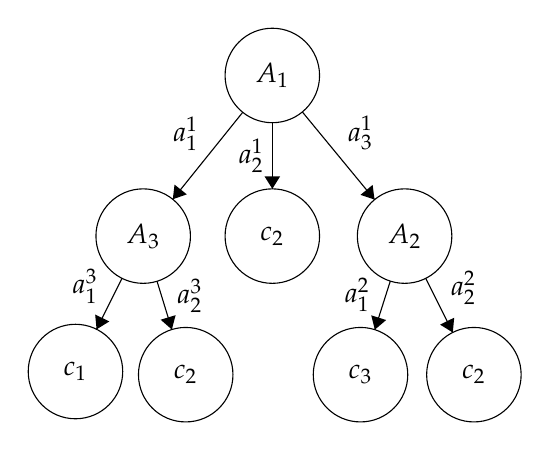
\begin{tikzpicture}[scale=0.2]
\tikzstyle{every node}+=[inner sep=0pt]
\draw [black] (18.1,-4.4) circle (3);
\draw (18.1,-4.4) node {$A_1$};
\draw [black] (9.9,-14.6) circle (3);
\draw (9.9,-14.6) node {$A_3$};
\draw [black] (5.6,-23.2) circle (3);
\draw (5.6,-23.2) node {$c_1$};
\draw [black] (12.6,-23.4) circle (3);
\draw (12.6,-23.4) node {$c_2$};
\draw [black] (18.1,-14.6) circle (3);
\draw (18.1,-14.6) node {$c_2$};
\draw [black] (26.5,-14.6) circle (3);
\draw (26.5,-14.6) node {$A_2$};
\draw [black] (23.7,-23.4) circle (3);
\draw (23.7,-23.4) node {$c_3$};
\draw [black] (30.9,-23.4) circle (3);
\draw (30.9,-23.4) node {$c_2$};
\draw [black] (16.22,-6.74) -- (11.78,-12.26);
\fill [black] (11.78,-12.26) -- (12.67,-11.95) -- (11.89,-11.33);
\draw (13.44,-8.08) node [left] {$a_1^1$};
\draw [black] (18.1,-7.4) -- (18.1,-11.6);
\fill [black] (18.1,-11.6) -- (18.6,-10.8) -- (17.6,-10.8);
\draw (17.6,-9.5) node [left] {$a_2^1$};
\draw [black] (20.01,-6.72) -- (24.59,-12.28);
\fill [black] (24.59,-12.28) -- (24.47,-11.35) -- (23.7,-11.98);
\draw (22.86,-8.07) node [right] {$a_3^1$};
\draw [black] (8.56,-17.28) -- (6.94,-20.52);
\fill [black] (6.94,-20.52) -- (7.75,-20.02) -- (6.85,-19.58);
\draw (7.05,-17.79) node [left] {$a_1^3$};
\draw [black] (10.78,-17.47) -- (11.72,-20.53);
\fill [black] (11.72,-20.53) -- (11.96,-19.62) -- (11.01,-19.91);
\draw (12.02,-18.37) node [right] {$a_2^3$};
\draw [black] (25.59,-17.46) -- (24.61,-20.54);
\fill [black] (24.61,-20.54) -- (25.33,-19.93) -- (24.38,-19.63);
\draw (24.33,-18.34) node [left] {$a_1^2$};
\draw [black] (27.84,-17.28) -- (29.56,-20.72);
\fill [black] (29.56,-20.72) -- (29.65,-19.78) -- (28.75,-20.22);
\draw (29.4,-17.89) node [right] {$a_2^2$};
\end{tikzpicture}
\caption{Example Decision Tree.}\label{fig:dt}
\end{center}
\end{figure}

Decision Trees are made recursively. First, attribute $i$ is chosen, and $D$ is partitioned into groups, one group for each element in $\mathcal{A}_i$. Then, the algorithm is recursively called on each subgroup. When some stopping criteria is met, such as a maximum depth being reached, a leaf is returned which contains some prediction in $\mathcal{C}$. Sometimes, many decision trees are made, and these predictions are aggregated by taking a vote. The general algorithm appears in Figure~\ref{fig:c45}.

The $\mathcal{A}_i$, $\mathcal{C}$, and $k$ are public information. Also, the budget used by recursive calls at the same recursive depth are disjoint. Thus, the total budget usage is
\[
\sum_{i=0}^k \max_{n \in \t{Nodes }n \t{on lvl }i} \epsilon_n
\]
where $\epsilon_n$ is the budget used on node $n$. It makes sense to use the same amount of budget for nodes on the same level, so this simplifies to $\sum_{i=0}^k \epsilon_{k}$.

There are three places that are unspecified in this general algorithm: The conditional that determines whether we stop growing the tree or not (Line 2, stopping criteria), the splitting column for each node (Line 7, greedy choice), and the number of trees in the forest (Line 14, number of trees). These choices are described below.
\begin{figure}

\lstinputlisting[style=MyPythonStyle, firstline=1, lastline=16]{./DTree.py}
\caption{Template for a decision tree algorithm. At Lines 2, 7, and 14, algorithmic choice can be made that change the performance.}\label{fig:c45}
\end{figure}

\subsection{Greedy Choice}
The way in which we choose the column on which to branch is a choice that exhibits data-dependence. Equivalently, we can view the problem as picking the attribute that maximizes the reduction in a potential function. The three choices we consider the Conditional Entropy, Gini coefficient, and the Max Operator~\cite{Friedman:2010}. To describe them, we use the following notation:
We denote by $\tau^{(i)}_{x}$ to be the number of elements of $D$ which have attribute $j$ on column $i$ and $\tau^{(i)}_{x,y}$ to be the number of elements which have attribute $j$ and on column $i$ and class $y$.
Then, the three values are:
\begin{align}
H_i(D) &= \sum_{j\in \mathcal{A}_i}\sum_{c \in \mathcal{C}} {\tau^{(i)}_{j,c}}\ln\left(\frac{\tau^{(i)}_{j}}{\tau^{(i)}_{j,c}}\right) \label{eq:ent} \\
G_i(D) &= \sum_{j \in \mathcal{A}_i} \tau^{(i)}_j\left(1-\sum_{c \in C}\left(\frac{\tau^{(i)}_{j,c}}{\tau^{(i)}_{j}}\right)^2\right)\label{eq:gini} \\
M_i(D) &= \sum_{j \in \mathcal{A}_i} \max_c(\tau^{(i)}_{j,c})
\label{eq:max}
\end{align}

Conditional entropy is the most widely-used potential function in practice, but in the private version, sensitivity comes into play. The sensitivities of the functions are described in the table below:
\begin{center}
\begin{tabular}{|l|l|}
\hline
Name & Sensitivity \\ \hline
Conditional Entropy & $\log(N+1) + \frac{1}{\ln(2)}$ \\ \hline
Gini Index & 2 \\ \hline
Max Opertator & 1 \\ \hline
\end{tabular}
\end{center}
Because the latter two functions have lower sensitivities, less noise must be added to them to make them $\epsilon$-DP per the exponential mechanism. For example, suppose we are choosing between columns $i$, $j$, and $k$ with scores $(3,2,-1)$ for some scoring function. Suppose that the scores under $H_i$ are $(3.1, 1.9, -1.1)$ and that the scores under $G_i$ are $(2.7, 2.2, -0.5)$. Even though $H_i$ is closer in value to the scoring function, its sensitivity is higher. If we have 100 database rows, the sensitivity of $H_i$ is 4.6 compared to 2 for $G_i$. Under 2-DP, the exponential mechanism releases $(i,j,k)$ with probability $(0.46, 0.35, 0.19)$ under $H_i$ and with probability $(0.5, 0.39, 0.11)$ under $G_i$. The expected score of the released answer is 1.9 for $H_i$ and 2.2 for $G_i$. This is an example of how high sensitivity can kill the accuracy of a function when $\epsilon$ is somewhat low.

One last important choice stems from the non-private machine learning literature: picking a random column. This results in less budget expenditure but obviously may lead to poor results. For this reason, random column selection is often combined with multiple trees~\cite{Jagannathan:2009}.

\subsection{Stopping Criteria}
The stopping criteria, or deciding when to make a leaf rather than branch, is another data-dependent choice. Stopping criteria are important to avoid overfitting when there isn't sufficient data in the branch. Having small amounts of data is also susceptible to the noise that DP adds, as relative error goes way up. There are a number of methods in the literature for deciding when to stop~\cite{Fletcher:2016}, and they can be classified into methods that don't use budget and methods that do.
\paragraph{No Budget Use} Without using budget, a ``global'' maximum depth must be used because the data can never be looked at. Maximum depth is a quantity that specifies the maximum recursion depth, or number of branches allowed to be taken before a leaf must be returned. This quantity can be user-specified or based on public information from the database, and we discuss the latter method. Borrowing from rules-of-thumb from non-private data mining, one method is $\frac{k}{2}$ where $k$ is the number of columns in the database. Another method which needs only the size of the initial database $|D|$ is to estimate the branching factor of the decision tree
\[
b = \frac{1}{k}\sum_{i=1}^k|\mathcal{A}_i|
\]
and then to set depth to be $\log_b(D)-1$.
\paragraph{Budget Use} This method queries the database at each branch. The noisy size $n$ of the database is computed privately, and the node is turned into a leaf if
\[
\frac{|D|}{t|C|} < \frac{\sqrt{2}}{\epsilon}
\]
where $t = \max_{i=1}^n|A_i|$. The LHS is an estimation of the signal, or number of points, that a leaf would calculate in each class. If the signal is less than $\frac{\sqrt{2}}{\epsilon}$, the variance of the Laplace distribution, then the calculation stops.

\subsection{Number of Trees}
A random decision forest can drastically outperform a single decision tree~\cite{Fletcher:2016}, and the number of trees in the forest is a data-dependent question. Uniquely in the private setting, if we train $\tau$ trees, we must use $\frac{\beta}{\tau}$ budget for each tree as the trees work on the same dataset. Thus, the number of trees can improve results, but too many trees will harm tree accuracy too much. Also, it even makes sense to have forests for private greedy trees as private trees are inherently random. To ensure tree diversity, it is often forced that each column appear as a member of the first branch an equal number of times, so each column appears approximately $\frac{\tau}{k}$ times in a first branch total.

Once all algorithmic choice has been made and a leaf has been returned, a noisy max over the class counts with the remaining budget is predicted.
Five instantiations of our general decision tree algorithm proposed by other authors are described in Figure \ref{fig:algtable} along with their budgets at each step.

\begin{figure}
\begin{center}
\begin{tabular}{|p{2cm}|p{3cm}|l|p{3cm}|l|p{1cm}|}
\hline
Paper & Stopping Criteria (Line 2) & $\epsilon_{stop}$ & Non-Leaf-Queries (Line 7) & $\epsilon_{NLQ}$ & $\tau$ (L.10) \\ \hline
Friedman \& Schuster~\cite{Friedman:2010} & $d$ user-defined; stop if $\frac{|D|}{t*|C|} < \frac{\sqrt{2}}{\epsilon_{\t{stop}}}$ & $\frac{\beta}{2d}$ & exp. mech with entropy& $\frac{\beta}{2d}$ & 1 \\ \hline
Mohammed et al.~\cite{Mohammed:2015} & $d$ user-defined & 0 & exp. mech with entropy & $\frac{\beta}{d}$ & 1 \\ \hline
Jagannathan et al.~\cite{Jagannathan:2009}, Fletcher \& Islam~\cite{Fletcher:2015} & $d=$ min of $\frac{k}{2}$ and $\log_b(|D|)-1$ & 0 & random & 0 & $\sim 10$ \\ \hline
\end{tabular}
\end{center}
\caption{Instantiations of the algorithm in Figure~\ref{fig:c45}. The total budget is $\beta$. The variable $d$ is the maximum depth that each algorithm uses to compute the budgets at each step.}\label{fig:algtable}
\end{figure}

\section{Experimental Setup and Hypotheses}

The code setup is presented in Figure~\ref{fig:dtree_choices}. We supply it choices, training databases, metafeatures, and models; we give details and justification below.
\paragraph{Choices} We consider only the three decision tree algorithms outlined in Figure \ref{fig:algtable} which we call Algorithms 1, 2, and 3. In Algorithm 1, we set the maximum depth to be 5 always, though the maximum height is rarely reached in most cases because of the additional stopping criteria. In Algorithm 2, we set the maximum height depending on the database size and branching factor in the same way as Algorithm 3, as we believe this is a good rule of thumb. We include three versions of Algorithm 3 with 1, 3, and 7 trees in a forest. We believe choosing among these five algorithms is a complex problem that involves both parameter optimization as well as a diverse set of algorithms.
\paragraph{Training Databases}
We used a combination of real and synthetic databases. Our databases consist of four large, real-world databases with discrete values. Their specifications are included in Figure~\ref{fig:dbinfo}. To obtain more database coverage, we included subsets of this database: We sampled between 20 and 100\% of the points and cut off from 0 to 75\% of the columns at random, repeating 100 times for each database. This results in 400 unique databases in total. 

We also generated synthetic datasets in the following way: we fixed between 5 and 10 columns to generate, fixed between 500 and 5000 points, and fixed the distributions of the attributes in each column. Then, we started forming a decision tree by picking a random column, splitting the database according to the column's attribute distribution, and recursing. After recursing twice, a new branch turns to a leaf with probability $p$ between 0.3 and 0.7. When a leaf is formed, a random element in the class is inputted for the class column, and unused columns are filled in randomly. This strategy is similar to the generation strategy used in~\cite{Friedman:2010}. We chose to use synthetic datasets generated from decision trees to simulate a more ideal, diverse training set for \Jostle{}. We generated 400 synthetic datasets in this manner.

\paragraph{Metafeatures} We use the following metafeatures: Log of number of rows in the database $\log_{10}(|D|)$, log of the product of the domain size $\log_{10}\left(\prod_{i=1}^k|\mathcal{A}_i|\right)$, the log of the number of classes $\log_{10}(|C|)$, and epsilon. We highlighted the impact of these metafeatures on performance in Section \ref{sec:pdtrees}.

\paragraph{Model} 
The model we used was regular decision trees, chosen because of their high interpretability in feature selection. The score function was a simple percentage of points in the test set that were incorrectly classified. The training to test split was 70/30. The output we sought was the best algorithm to use. Once our decision tree picked an algorithm, we dispatched the algorithm (with the proper reduction in $\epsilon$ for metafeatures) and computed the error.
\begin{figure}
\begin{center}
\begin{tabular}{|p{3cm}|l|l|l|l|}
\hline
Name & No. Points & No. Cols & Avg. Branch Size & Class size \\ \hline
Protease C & 1625 & 8 & 20 & 2 \\ \hline
Nursery & 12960 & 8 & 3.375 & 5 \\ \hline
Tic-tac-toe & 958 & 9 & 3 & 2 \\ \hline
Student Loan & 1000 & 8 & 6.125 & 2 \\ \hline
\end{tabular}
\end{center}
\caption{Specifications of the four real-world databases used for training.}\label{fig:dbinfo}
\end{figure}

We split the 600 databases into a training set which we fed to the \t{ChoiceMaker} and a testing set which we treated as being private databases on which the \t{ChoiceMaker} actually made a choice. For every element in the test set, we computed the performances of the five decision tree algorithms and the model we learned, and computed regret: the error relative to the highest-performing algorithm in hindsight, averaged over all databases in the test set.

We chose the following ratios of synthetic and real datasets for two different scenarios:

\begin{center}
\begin{tabular}{|p{2cm}|p{2cm}|p{2cm}|p{2cm}|p{2cm}|}
\hline
\; & Train Synthetic Pct. & Train Real Pct. & Test Synthetic Pct. & Train Real Pct. \\ \hline
Scenario 1 & 75 & 75 & 0 & 25 \\ \hline
Scenario 2 & 75 & 0 & 25 & 0\\ \hline
\end{tabular}
\end{center}
We believe the scenarios have the following properties:
\begin{itemize}
\item{Scenario 1: This test has a diverse set of training databases and a real-world output dataset in its training set. The testing set consists of one entire real-world dataset that doesn't appear in the training data. This is the most realistic version of \Jostle{} where the test set contains private data that haven't been seen before.}
\item{Scenario 2: This test presents an idealized \Jostle{} situation: the training and test sets look very similar. In the real world, this may not always happen because such high-quality data doesn't always exist.}
\end{itemize}
Our hypotheses are the following:
\begin{itemize}
\item For Scenario 1, \Jostle{}'s regret may be lower than any individual algorithm, and if not, it will be due to properties in the training set.
\item For Scenario 2, \Jostle{}'s regret will be much lower than other algorithms because the training and testing set are similar.
\end{itemize}
%Say results up front.
\section{Results}
\begin{figure}
\begin{center}
\includegraphics[scale=0.8]{Results}
\end{center}
\caption{Top: Scenario 1's regret as a percentage, minus 100. Bottom: Scenarios 2's regret as a percentage, minus 100.}
\label{fig:results}
\end{figure}
For Scenario 1, we collected four runs, putting each of the four real databases entirely in the validation set each time, and computed the average regret. Our results on the two scenarios are plotted in Figure~\ref{fig:results}. We can see that for Scenario 3, the model's regret of 1.02 is significantly lower than the rest of the databases as expected. In Scenario 1, Algorithm 1~W\cite{Friedman:2010} outperforms our model, but we still do better than the other models. This could be due to the following reasons:
\paragraph{Different performance properties of the algorithms} The data in Scenarios 1 and 2 are inherently different, and causes the algorithms to perform different relatively to each other. In Scenario 1, Algorithm 1 outperforms other models by a more significant margin compared to Scenario 2. Algorithm 1's regret is 1.13 and the second-place Algorithm 3 on 7 trees is 1.19 whereas in Scenario 2, the first- and second-place algorithms perform comparably at 1.06 and 1.07. 
\paragraph{Differences in the training and testing set} As mentioned before, Scenario 2 is a more idealized execution of \Jostle{} because the train and test sets are drawn from the same distribution. In Scenario 1, the test set is a distribution never seen in the training set because it's treated like a private dataset.

Our data support the second part of our hypothesis. The first part is not proven or disproven by our results; more experiments are needed to examine the problem. However, it's likely to have been caused by some combination of the two reasons above, and we discuss these implications more in the conclusion.

\chapter{Conclusions and Future Work}\label{ch:future}
\section{Conclusions}
The purpose of \Jostle{} is to provide the first tool for making algorithmic choice in its full generality. This is a difficult problem because experimentation can never be fully automated, and a tradeoff between automating as much as possible while still making optimal decisions must be made. \Jostle{} makes this tradeoff by proposing the \t{ChoiceMaker} construct which performs meta-machine learning on metafeatures from the database in an automated way. We evaluated this design by performing the first automated algorithmic choice for private decision trees, an example that previous approaches aren't general enough to tackle.
We found that \Jostle{} is capable of making the best choice quite often in some cases, but in other cases, its performance can be limited.

There are a few reasons behind this limitation. First, the data on which \Jostle{}'s model is trained may be quite different from what the private database looks like when actually running the algorithm. Second, the metafeatures may provide little insight into algorithmic choice. Third, the model may be ill-suited to nature of the learning problem, like trying to fit a linear regression to a vary wavy curve. We believe that all three of these reasons could have caused \Jostle{} to not outperform one of the algorithms in one of our tests.

However, we argue that the only fix to these limitations is to use higher-quality data science techniques which is a very hard problem to automate. If a programmer inputs poor metafeatures, then it would be difficult indeed to write any algorithm that will fix them. The empirical nature of the general algorithmic choice problem necessitates some level of data science effort to judge if the meta-machine learning is tractable and how to fix it if not. We believe that the current frontier of research for this problem will be to explore different setups for algorithmic selection constructs (other than \t{ChoiceMaker}) or to incorporate some data science tools to help the programmer do data science more easily.
%How well decision trees will generalize.
\section{Future Work}
Here, we discuss future work for \Jostle{}. We hope to extend \Jostle{} in the following areas: automation, performance optimization, and experiment extent.
\subsection{Automation}
\Jostle{} does remove the necessity of finding necessary data science from the programmers The insights gleamed will only be as powerful as the input metafeatures and any feature-selection done by the \t{Model} during training, so a programmer must still do some analysis before using a \t{ChoiceMaker}. Suppose we have the following metafeatures (which were considered for the decision tree experiment):
\begin{lstlisting}[style=MyPythonStyle]
uniformity = Metafeature(data){
    db = data.database
    xgrp = sqrt(db.x_range)
    ygrp = sqrt(db.y_range)
    return {{stddev(select sum(values) from db 
                    groupby x/xgrp, y/ygrp)}}
}
sparsity = Metafeature(data){
    db = data.database
    num_nonzero = {{select count(values) from db 
                    where values > 0}}
    domain_size = db.x_range * db.y_range
    return num_nonzero/domain_size
}
\end{lstlisting}

A programmer would need to have some insights in order to propose these rather-complex metafeatures to a \t{ChoiceMaker}. The analysis contributes to programmer overhead, and perhaps the programmer has made a suboptimal metafeature. To solve this problem, we hope to use algorithm synthesis in the \t{Model} to reduce the complexity of the \t{Metafeatures}. Suppose that, instead of inputting the exact uniformity definition, a programmer indicates the simpler metafeature:
\begin{lstlisting}[style=MyPythonStyle]
uniformity = Metafeature(data){
    db = data.database
    xgrp = sqrt(db.x_range)
    ygrp = sqrt(db.y_range)
    return {{select sum(values) from db 
                    groupby x/xgrp, y/ygrp}}
}
\end{lstlisting}
Instead of returning a real number, an entire database is returned. Instead of learning a regression on the metafeatures, the \t{Model} would learn SQL expressions to aggregate the metafeature databases into a real number. Perhaps it learns that the most suitable aggregation to use is average deviation as opposed to the programmer-specified \t{stddev}. Synthesis can also make edits, too: perhaps instead of using a bucket size of $\sqrt{\t{db.x\_range}}$, a better exponent is $(\t{db.x\_range})^{0.4}$. We find it promising that synthesis for noisy input-output pairs has been done already with deep neural networks \cite{Devlin:2017}, at least when generating a program from scratch as opposed to editing.

\subsection{Global Optimization}
\Jostle{} and Pythia both optimize greedily, and there is likely opportunity to greatly improve the performance of \Jostle{}. We say the optimization is greedy because \t{ChoiceMakers} act independently of each other, making the best decisions for themselves but not for the program as a whole. Consider the following juxtaposed \t{ChoiceMakers}:
\begin{lstlisting}[style=MyPythonStyle]
noisyHistChoice = MkChoiceMaker among {DTreeAlg1, DTreeAlg2}
                    informed by {uniformity, sparsity}
                    trained on trainingSet 
                    wrt ScoreFunc
linRegression = MkChoiceMaker among {LinReg(0.1), LinReg(1)}
                    informed by {size}
                    trained on trainingSet
                    wrt ScoreFunc2
def get_answers(db, y_pts):
    q_answers = noisyHistChoice(db)
    db_mod = modify db using q_answers
    reg_model = linRegression(db_mod)
    return reg_model.predict(y_pts)
\end{lstlisting}
\Jostle{} currently works by optimizing the first and then the second \t{ChoiceMaker}. This is problematic since linRegression depends on an output from noisyHistChoice. The score function of NoisyHistChoice should reflect that it's being fed into linRegression, but it may not and the programmer may not know how to choose the score function. A better way of doing this calculation would be to squish the two \t{ChoiceMakers} together like
\begin{lstlisting}[style=MyPythonStyle]
linRegression = MkChoiceMaker among {(DTreeAlg1, LinReg(0.1)),
                                    (DTreeAlg2, LinReg(0.1),
                                    (DTreeAlg1, LinReg(1)),
                                    (DTreeAlg2, LinReg(1))}
\end{lstlisting}
This transformation could be made automatically as an optimization by \Jostle{} and would result in a more globally-optimal algorithm.
\subsection{Experimental extent}
We would like to do more experiments in the areas of utility functions and hyperparameter optimization. 

Utility functions are used in the exponential mechanism. Some utility functions, like conditional entropy on decision trees, are empirically known to perform the best in the non-private setting. However, in the private setting, an important consideration is the sensitivity of the utility function; if a less-utile function has less sensitivity, then less noise will interfere with its answer. In addition to decision trees, private causal inference exhibits this problem \cite{Kusner:2016}.
\bibliographystyle{plain}
\bibliography{Thesis}
\end{document}